\documentclass[a4paper,10pt]{article}
\usepackage[margin=1.5cm]{geometry}

\usepackage{graphicx}
\usepackage[no-math]{fontspec}

\usepackage{fontspec} % For loading fonts
\defaultfontfeatures{Mapping=tex-text}
%\setmainfont{Segoe UI Semilight} % Main document font

\usepackage{xunicode,xltxtra,url,parskip} % Formatting packages

\usepackage[usenames,dvipsnames]{xcolor} % Required for specifying custom colors

\usepackage[big]{layaureo} % Margin formatting of the A4 page, an alternative to layaureo can be \usepackage{fullpage}
% To reduce the height of the top margin uncomment: \addtolength{\voffset}{-1.3cm}
\addtolength{\hoffset}{-1cm}

\usepackage{titlesec} % Used to customize the \section command
\titleformat{\section}{\Large\scshape\raggedright}{}{0em}{}[\titlerule] % Text formatting of sections
\titlespacing{\section}{0pt}{20pt}{3pt} % Spacing around sections

\usepackage[ngerman]{babel} 

\usepackage{tabularx}
\usepackage{hyperref}
\usepackage{fancyhdr, xcolor}
\fancyhf{} %deletes default header and footer settings
\renewcommand{\headrulewidth}{0pt} %no header line

\usepackage{fontspec,xltxtra} %fonts and styles in xelatex
% \setmainfont{Linux Libertine O}
\usepackage{fontawesome5}
\usepackage{raleway}                      % Load raleway font
\renewcommand{\familydefault}{\sfdefault} % Set sans serif for document

\fancyhead[C]{\footnotesize{\color{gray}{\faUser \hfil Giovanni Perez Montt \hfil|\hfil \faMapMarker \hfil Aretzstr. 52, 52070 Aachen \hfil|\hfil \faEnvelopeOpen  \hfil giovanni.perez.montt@gmail.com \hfil|\hfil \faPhone \hfil +49 157 72192486 }}}

\usepackage{tikz}
\usetikzlibrary{positioning,fit,calc}
\usetikzlibrary{arrows}
%--------------------------------------------------------------------------------------

\begin{document}
\newcolumntype{L}[1]{>{\raggedright\arraybackslash}p{#1}}
\newcolumntype{R}[1]{>{\raggedleft\arraybackslash}p{#1}}

\pagestyle{fancyplain} %apply customized header to all pages
\thispagestyle{empty} % no header on this page

%--------------------------------------------------------------------------------------
% Deckblatt
%--------------------------------------------------------------------------------------
%
\begin{minipage}[t][5cm][b]{\textwidth}
\begin{center}
\hspace{1cm}\\
\Huge\textsc{DevOps Engineer /}\\
\Huge\textsc{System Integrator}\\
\vspace{0.5 cm}


\hspace{2cm}\\
\huge\textsc{Osthus GmbH}\\
\end{center}
\end{minipage}

\vfill
\begin{center}
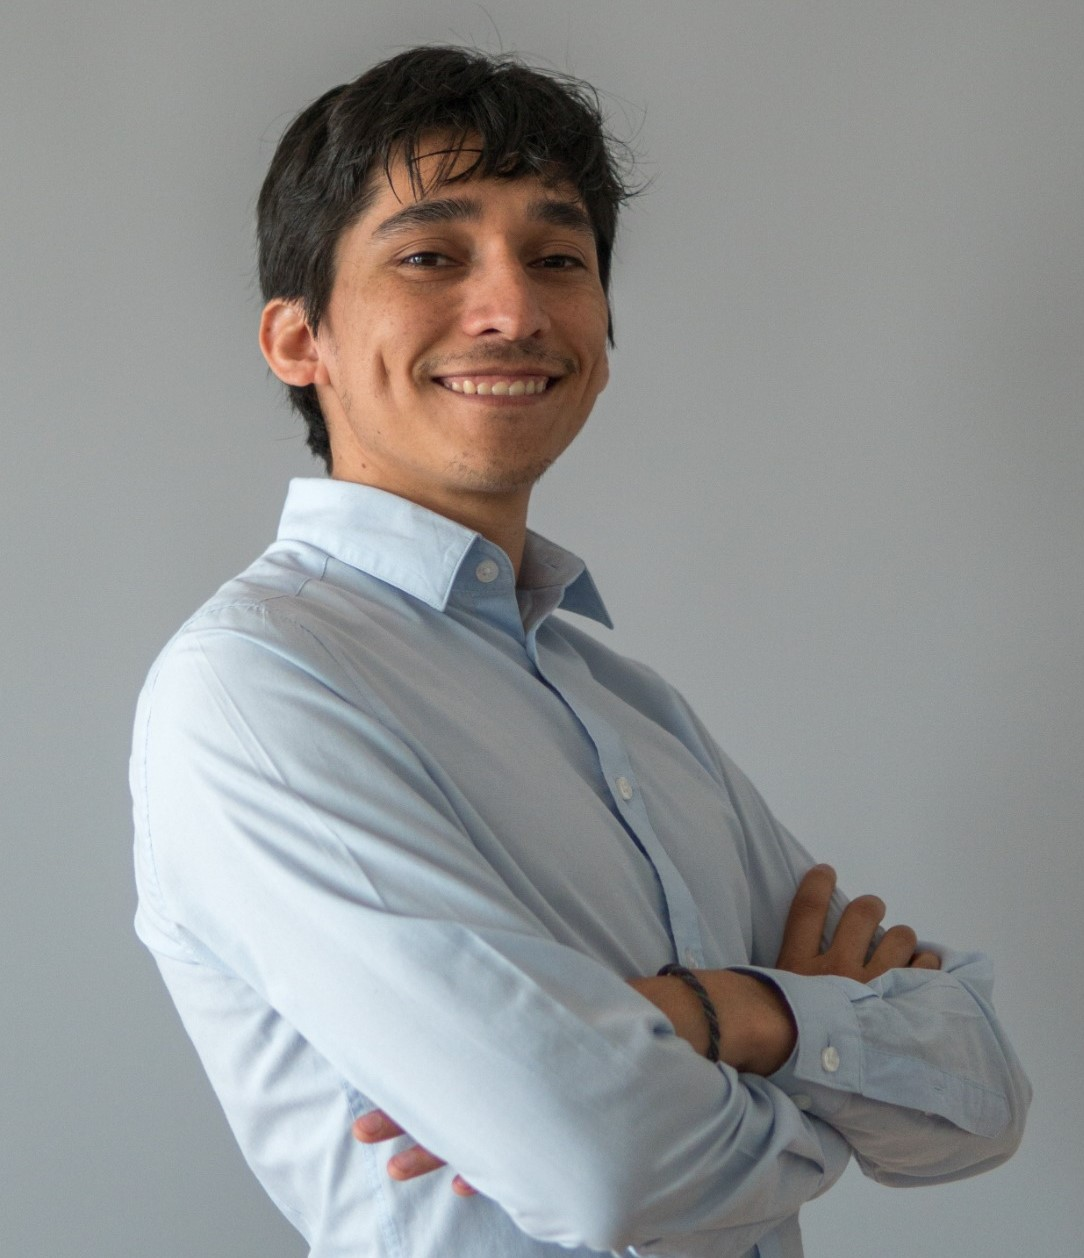
\includegraphics[width=0.7\textwidth]{pics/profilegio3.jpeg}
\end{center}
\vfill

\begin{minipage}[b][5cm][t]{\textwidth}
\centering\Large
\textsc{Giovanni Perez Montt}\\
\textsc{\faGraduationCap {Elektrotechniker (Diplom)} }\\
\vspace{0.5cm}
\textsc{\faMapMarker Aretzstr.  52  \\ 52070 Aachen}\\
\textsc{ \faEnvelopeOpen giovanni.perez.montt@gmail.com}\\
\textsc{\faPhone +49 157 5356 9384 }
\end{minipage}
\newcolumntype{L}[1]{>{\raggedright\arraybackslash}p{#1}}
\newcolumntype{R}[1]{>{\raggedleft\arraybackslash}p{#1}}

\pagestyle{fancyplain} %apply customized header to all pages
\thispagestyle{empty} % no header on this page


% \begin{tikzpicture}[remember picture, overlay]
%   \draw[line width = 2pt] ($(current page.north west) + (1in,-1in)$) rectangle ($(current page.south east) + (-1in,1in)$);
% \end{tikzpicture}

%---------------------------------------------------------
%------
%------------------------
\pagebreak

\pagestyle{fancyplain} %apply customized header to all pages

\begin{infoEnterprise}
OSTHUS GmbH \\
Eisenbahnweg 9-11 \\
52068 Aachen 
\end{infoEnterprise}

\begin{dateofdocument}
\hfill
Aachen, den \today
\end{dateofdocument}
\vspace{0.05cm}
\\


%%----------Betreff
\begin{page}{\textwidth}
\textbf{Bewerbung als DevOps Ingenieur / System Integrator} \vfill
Sehr geehrte Frau Braun,\vfill

auf Empfehlung Ihrer Kollegin Dr. Jennifer Aschenbrenner wurde ich auf die Stelle System Integrator aufmerskam. Ich informierte mich weiter und stieß auf die Ausschreibung DevOps Engineer, welche ebenfalls mein Interesse weckte. Ich möchte hiermit die Gelegenheit nutzen mich und meine Hintergründe kurz vorzustellen und potenziell auf beide Stellen zu bewerben. 

Ich bin Elektrotechniker (chilenisches Diplom mit Schwerpunkt Robotik und Regelungstechnik). Während des Studiums bearbeitete ich bereits private Projekte (Microcontroller, Sensoren, hardwarenahe Programmierung) in Folge erfolgreicher Forschungsanträge. 2013 führt mich meine Technologie- und Innovationsorientierung als Austauschstudent (Stipendiat DAAD) nach Deutschland.\vfill

Seit 2015 bin ich auf eigene Faust in Deutschland; getrieben vom Wunsch, langfristig als innovativer Ingenieur Fuß zu fassen. Teils als studentische Hilfskraft, teils als Freiberufler erlebte ich aus der Nähe mit, dass im Bereich der Automatisierungstechnik, Robotik und Industrie 4.0 mehr erforderlich ist als eine Vision aus Elektrotechniker-Sicht. Seit 2015 arbeitete ich routinemäßig unter Unix und rutschte seitdem immer weiter in die Softwareentwicklung, die mich bis heute fasziniert. Erwähnenswert ist hier meine Arbeit am Maskor Institut der FH Aachen (ROS, Microntroller, Sensorintegration). \vfill
 
Es macht mir großen Spaß, das Gesamtpaket eines Projekts zu erleben und bei der kreativen Planung bis zur praktischen Ausführung vorne mit dabei zu sein. In diesem Rahmen unterstütze ich die 3D Punkt LSL UG seit Gründung als fester Innovationspartner, insbesondere als Software-Architekt für Embedded Systems. Bei meinem aktuellen Arbeitgeber Velocity Mobility GmbH implementierte ich kürzlich ein GPS-Tracking System inkl. Datenbank im Fahrrad-Verleihsystem mithilfe von Docker. Zuvor war ich an der Entwicklung von verschiedenen Softwareprojekten (Python/Bash Scripts, Umgebungstools, Build System, Netzwerke und Deploying der Software) beteiligt. Im vergangenen Jahr sammelte ich intensiv Kenntnisse in CI, Versionierung, Software Release und Deployment.  \vfill

Da ich in interdisziplinärer Arbeit aufgehe, sagt mir ihr vielvältiges Firmenprofil sehr zu. Insbesondere freue ich mich auf eine sich ständig verändernde, herausfordernde, und innovative Arbeitsumgebung. Ihre gelebte Teamorientierung passt genau zu meinem Profil. Meine Kundenorientierung habe ich sowohl bei 3D Punkt als auch Velocity als Korrespondent für internationale Kunden unter Beweis gestellt.\vfill
Sie werden in mir einen überdurchschnittlich engagierten, kollegialen und teamfähigen Ingenieur kennenlernen. Ich lerne sehr schnell (außer Fremdsprachen) und arbeite gerne autodidaktisch. Seit der bekannten Home Office Krise fülle ich meine Freizeit mit Online-Kursen über Datenbanken und Java Script. Ich habe großes Interesse daran, mich professionell als Softwareentwickler zu profilieren. Die Stelle System Integrator kann ich mir daher gut vorstellen. Noch mehr reizt mich persönlich die Stelle DevOps Engineer, mit der ich direkt auf meine aktuellen spannenden Tätigkeiten aufbaue. \vfill

Ich freue mich auf eine kurzfristige Einladung zum persönlichen Kennenlernen, um Sie von meiner
hohen Motivation und meiner Lust am Lernen zu überzeugen. Bis dahin verbleibe ich\vfill
mit freundlichen Grüßen



\begin{minipage}[c][3cm][b]{4cm}
	
\includegraphics[width=0.7\linewidth]{pics/firma.png}
	\centering Giovanni Perez
\end{minipage}
\hfill
\begin{minipage}[c][3cm][b]{4cm}
\raggedleft { \textbf{Anlagen}}\\ \hspace{0.5cm}
Curriculum Vitae\\ Zeugnisse
\end{minipage}


\end{page}
\pagebreak


\end{document}

